\documentclass[aspectratio=169]{beamer}

\usetheme{boxes}
\useinnertheme{circles}

\definecolor{UC}{RGB}{0, 50, 98}
\definecolor{Beamer}{RGB}{51, 51, 178}
\definecolor{Hooker}{RGB}{73, 121, 107}
\definecolor{Triton}{RGB}{0, 106, 150}
\definecolor{Prussian}{RGB}{0, 49, 83}
\definecolor{Forest}{RGB}{101, 121, 48}
\definecolor{Metro}{RGB}{35, 55, 59}
\definecolor{Gamboge}{RGB}{228, 155, 15}
\definecolor{Devil}{RGB}{115, 39, 43}
\definecolor{Shade}{RGB}{250, 250, 250}
\definecolor{JPAL}{RGB}{227, 89, 37}
\definecolor{IPA}{RGB}{90, 128, 38}

\usecolortheme[named=Triton]{structure}

% \setbeamercolor{background canvas}{bg=Shade}
\setbeamercolor{block title}{bg=Beamer!12}
\setbeamercolor{block body}{bg=Beamer!8}

\setbeamersize{text margin left=0.2in,text margin right=0.2in}

% \setbeamertemplate{footline} % To remove the footer line in all slides uncomment this line
\setbeamertemplate{footline}[page number] % To replace the footer line in all slides with a simple slide count uncomment this line
\setbeamertemplate{navigation symbols}{} % To remove the navigation symbols from the bottom of all slides uncomment this line
\setbeamertemplate{bibliography item}{}
\setbeamertemplate{caption}[numbered]

\setbeamertemplate{frametitle}{%
    \usebeamerfont{frametitle} \vspace{0.5em} \insertframetitle%
    \vphantom{g}% To avoid fluctuations per frame
    \vspace{0.5em} \hrule% Uncomment to see desired effect, without a full-width hrule
    \par\hspace*{-\dimexpr0.5\textwidth-0.5\textwidth}\rule[0.5\baselineskip]{\textwidth}{0.4pt}
    \par\vspace*{-\baselineskip}% <-- reduce vertical space after rule
}

\usepackage[T1]{fontenc}
\usepackage{inconsolata}
% \usepackage[sfdefault,light]{roboto}
\usepackage{cmbright}
% \usepackage[default]{lato}
\usepackage{amsmath, amssymb, amsthm, mathrsfs, bbm}
\usepackage{threeparttable, adjustbox, tabularx, booktabs}
\usepackage{appendixnumberbeamer}
\usepackage{hyperref}
\usepackage{pdflscape}
\usepackage{placeins}
\usepackage{caption}
\usepackage{graphicx}
\usepackage{listings}
\usepackage{color,soul}
\usepackage{tfrupee}
\usepackage[backend=bibtex, style=authortitle, citestyle=authoryear-icomp, url=false]{biblatex}
\addbibresource{Lottery.bib}

\newcommand{\inv}[1]{#1^{-1}}
\newcommand{\iid}{\text{i.i.d.}}
\newcommand{\bmat}[1]{\begin{bmatrix} #1 \end{bmatrix}}
\newcommand{\asconv}{\xrightarrow{a.s.}}
\newcommand{\pconv}{\xrightarrow{p}}
\newcommand{\dconv}{\xrightarrow{d}}
\newcommand{\msconv}{\xrightarrow{m.s.}}
\newcommand{\liminfty}{\lim_{n \to \infty}}
\newcommand*\diff{\mathop{}\!\text{d}}
\newcommand{\lhood}{\mathcal{L}}
\newcommand{\var}{\text{Var}}
\newcommand{\ev}{\text{E}}
\renewcommand{\vec}[1]{\mathbf{#1}}
\newcommand{\specialcell}[2][c]{\begin{tabular}[#1]{@{}c@{}}#2\end{tabular}}

\newtheorem{prop}{Proposition}
\newtheorem{claim}{Claim}
\newtheorem{assume}{Assumption}
\newtheorem{define}{Definition}

\newenvironment{wideitemize}{\itemize\addtolength{\itemsep}{10pt}}{\enditemize}
\newenvironment{wideenumerate}{\enumerate\addtolength{\itemsep}{10pt}}{\endenumerate}

\let\oldforall\forall
\let\forall\undefined
\DeclareMathOperator{\forall}{\oldforall}
\DeclareMathOperator*{\argmax}{arg\,max}
\DeclareMathOperator*{\argmin}{arg\,min}

\lstset{
  basicstyle=\footnotesize\ttfamily,
  columns=fixed,
  fontadjust=true,
  basewidth=0.5em
}

\title{The Role of Regret in Prize-Linked Savings: Experimental Evidence from Kenya}
\author[Abraham, Akbas, Ariely, Jang]{Justin Abraham\inst{1} \and Merve Akbas\inst{2} \and Dan Ariely\inst{2} \and Chaning Jang\inst{3}}
\institute{\inst{1} University of California, San Diego \and \inst{2} Duke University \and \inst{3} Busara Center for Behavioral Economics}
\date{\today}

\begin{document}

\begin{frame}
	\titlepage
\end{frame}

\begin{frame}{Savings as a Policy Objective}

	\begin{wideitemize}

		\item Access to savings is an important avenue toward economic development.
		% Can be used to invest in productive assets when unable to
		% Allows for some degree of consumption smoothing when insurance is incomplete. 

		\item Poor households face savings constraints.

		\begin{itemize}
			\item Only 22 percent of the world's poorest have an account at a financial institution \parencite{demirguc-kunt_global_2018}. Even less use them regularly.
			\item The prevalence of alternative strategies (livestock, cash under the mattress, informal groups, gambling, etc.) suggest a latent demand for saving.
		\end{itemize}

		\item Product design (default savings, commitment devices, reminders) targeted to problems of self-control/attentiveness have proven very cost-effective \parencite{ashraf_tying_2006,dupas_why_2013,somville_saving_2018}.
		% In addition to supply-side interventions such as bank expansions and subsidies
		% Our paper sits among the research on demand-side frictions.

	\end{wideitemize}

\end{frame}

\begin{frame}{Prize-Linked Savings}

	Prize-linked savings (PLS) provide stochastic returns to savings deposits (a lottery ticket for saving).

	\begin{wideitemize}
		\item Typically returns full principal (no negative returns).
		\item Involves both in-kind and monetary rewards.
		\item Has existed since the 17th century and can be found in both the developed and developing world.
		\item There is policy interest in using this product as a way to encourage saving \parencite{kearney_making_2010}.
	\end{wideitemize}

\end{frame}

\begin{frame}{Research Questions}

	\begin{wideenumerate}

		\item Can prize-linked savings induce account usage in low-income settings?
		\item How much of this effect can we attribute to a specific mechanism (regret aversion)?

		% Why risk-averse people play the lotteries is a puzzle with a lot of explanations. Here we focus on one.

	\end{wideenumerate}

\end{frame}

\begin{frame}{Overview}

	\begin{wideitemize}

		\item Provided a mobile savings account to 311 periurban residents of Nairobi, Kenya.
		\item Experimentally vary the incentive structure (fixed versus stochastic) and information structure.
		\item Observe account activity over a 60-day period.

		\begin{enumerate}
			\item Estimate the effect of stochastic incentives on program savings and usage.
			\item Estimate the effect on savings by other means, consumption, and gambling.
			\item Quantify the role of regret aversion.
		\end{enumerate}

	\end{wideitemize}

\end{frame}

\begin{frame}{Study Setting}

	\begin{columns}

		\begin{column}{0.48\textwidth}

			\begin{itemize}
				\item Sample of 311 adults from Kibera and other settlements around Nairobi.
				\item Less than half of the sample consider themselves employed.
				\item Many are salespersons and casual laborers: only 5\% receive regular income with an average of USD PPP 77 monthly.
				\item A little over half save regularly and most use ROSCAs.
				\item Average savings amount to USD 23.
				\item 24\% report having gambling problems.
			\end{itemize}

		\end{column}

		\begin{column}{0.48\textwidth}

			\begin{figure}[H]
				\centering
				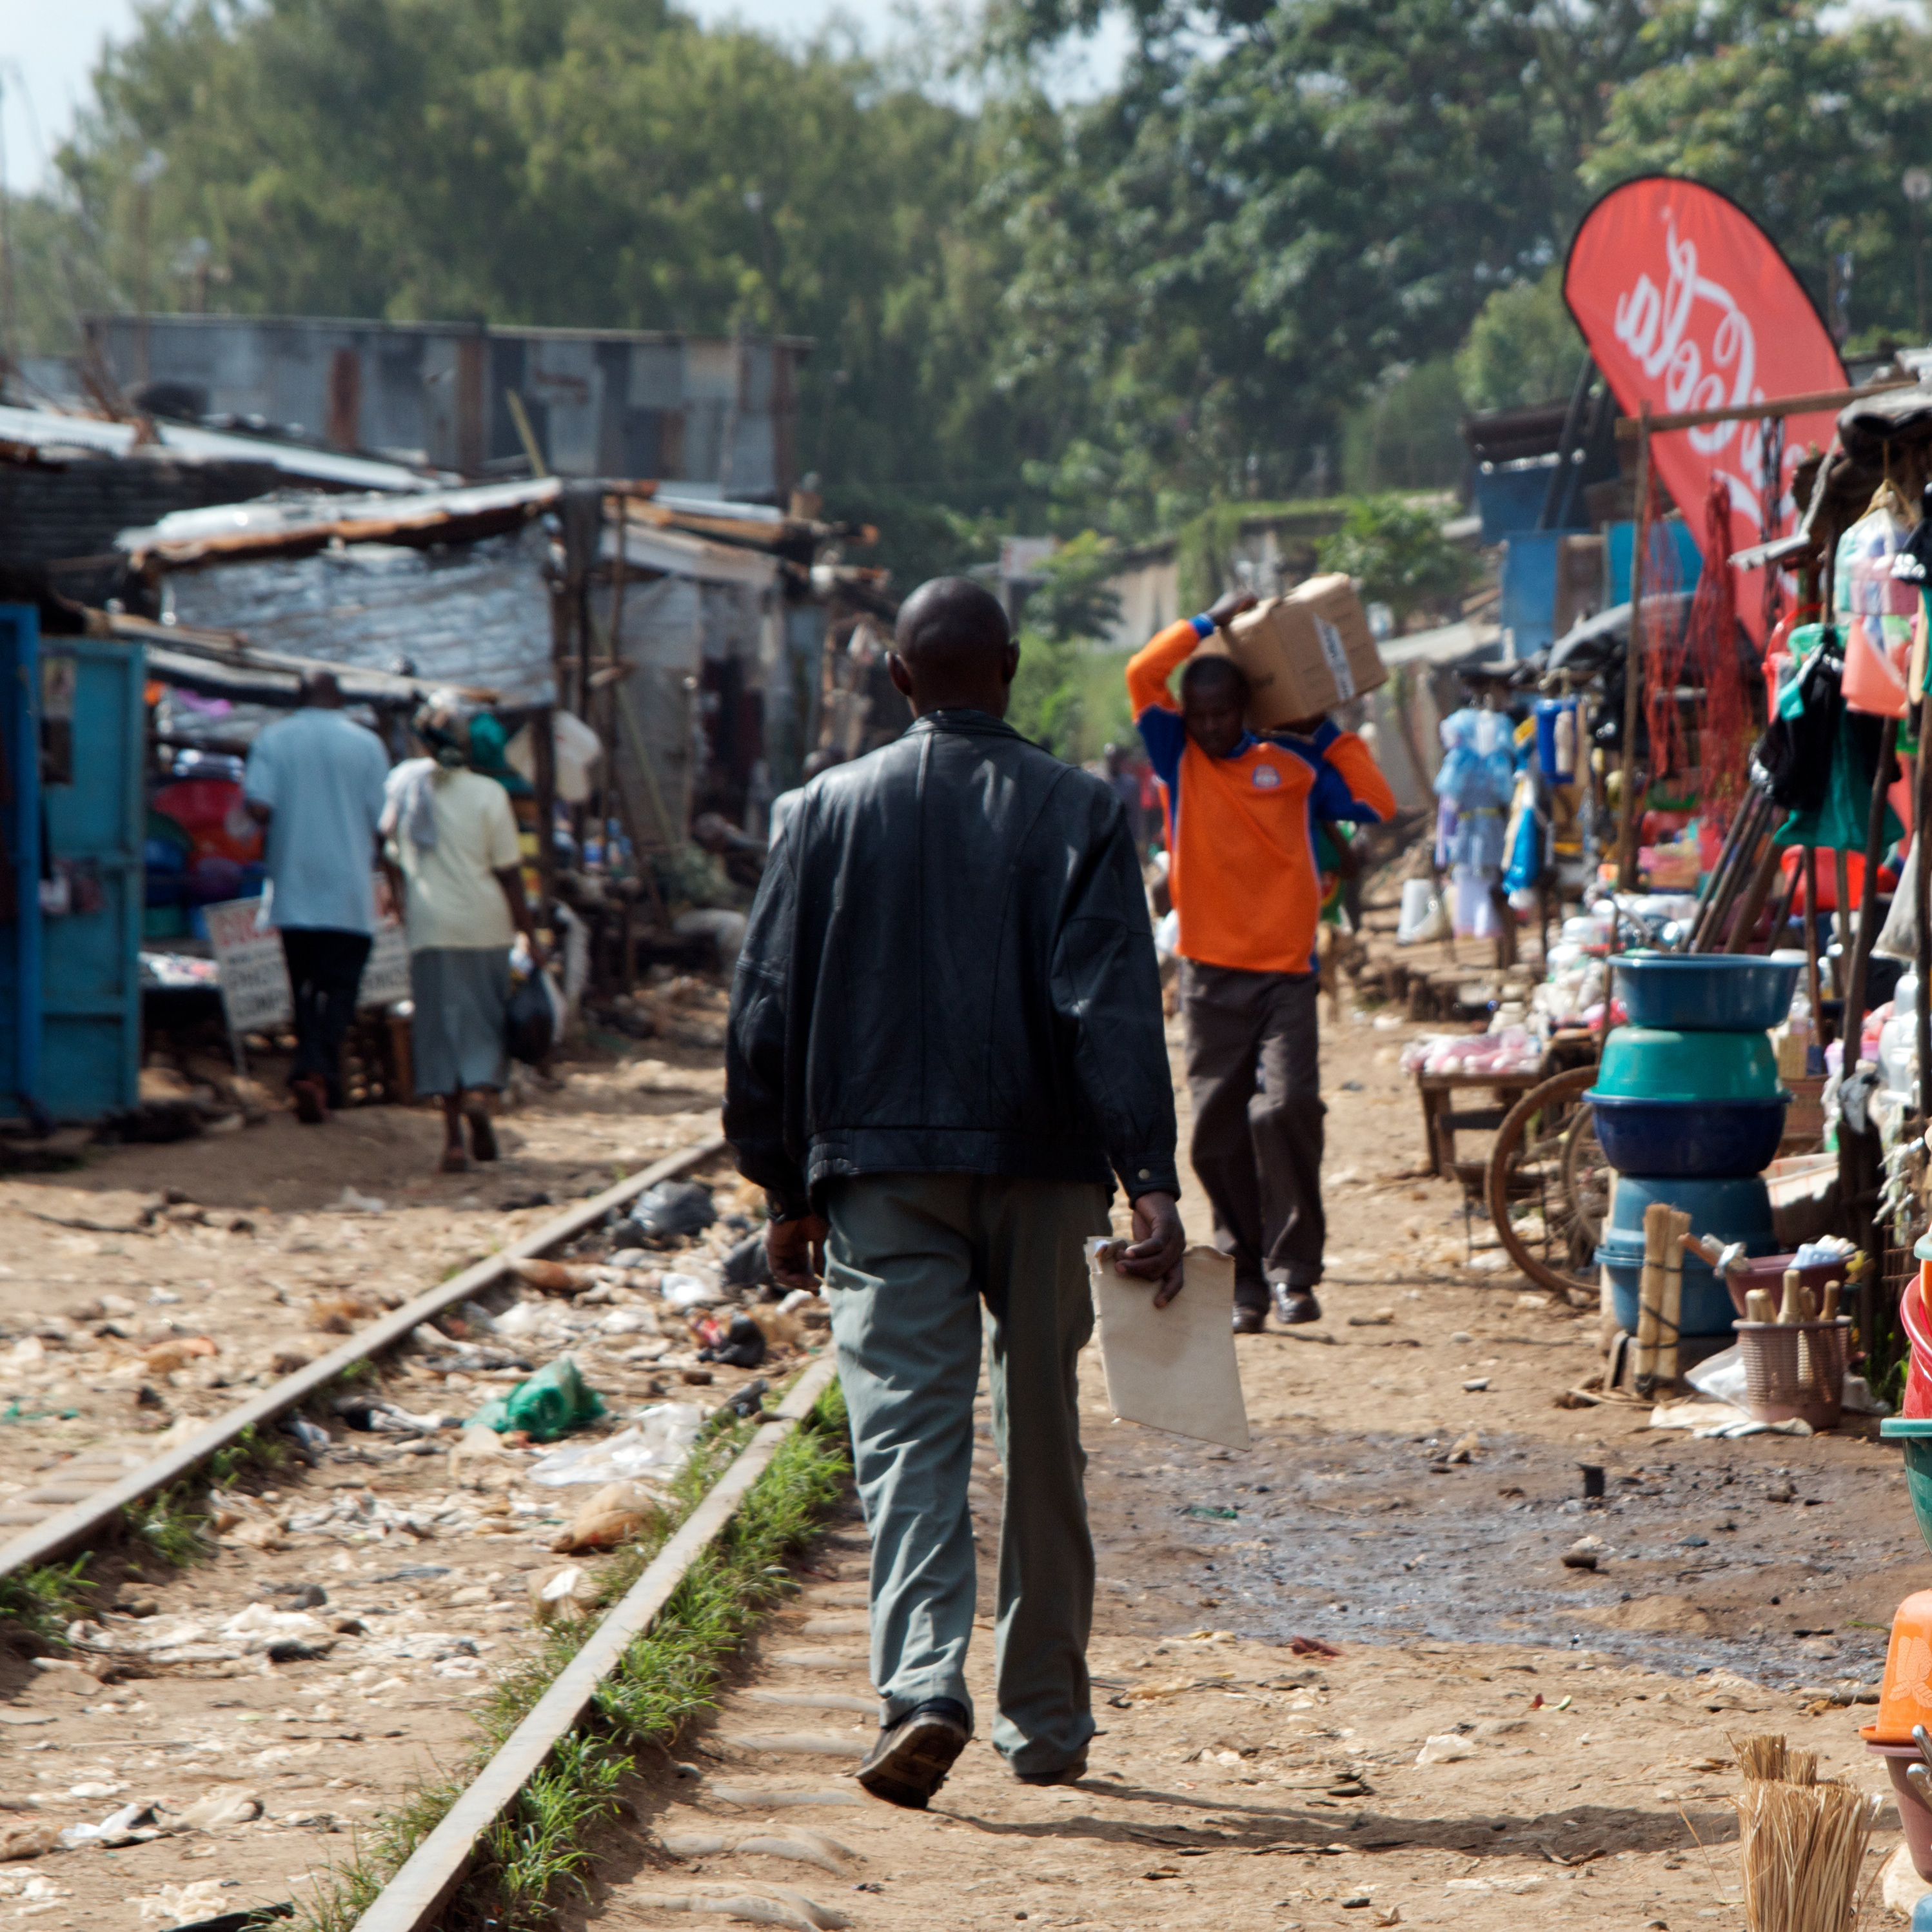
\includegraphics[height=0.8\textheight]{kibera-tracks-square.jpg}
			\end{figure}

		\end{column}

	\end{columns}

	% https://qz.com/africa/1140842/gambling-addiction-is-on-the-rise-in-kenya-and-leaving-young-people-bankrupt-and-suicidal/

\end{frame}

\begin{frame}{Mobile Savings}
	
	\begin{wideitemize}
		\item Subjects provided an airtime account linked to their mobile phones for 60 days.
		\item Transactions made by sending airtime free of charge.
		\item Subjects received daily SMS reporting balance.
		\item Lockbox savings; withdrawal allowed only on the 30th and final day.
		\item Principal and returns transferred to subjects after 60 days via M-Pesa.
	\end{wideitemize}

	% Everyone has a mobile phone, know how to use mobile money, cash out easily, high trust, in order to minimize the role of transaction costs/information/trust

\end{frame}

\begin{frame}{Experiment}

	\begin{block}{Control ($N = 105$)}
		\begin{itemize}
		\item Certain 5\% return applied to daily deposits
		\item Daily balance and returns reported via SMS
		\end{itemize}
	\end{block}

	% Important to use a standard account with equivalent expected returns so that we comapre only the effect of the stoschastic incentive

	\begin{columns}[T]

		\begin{column}{0.48\textwidth}
			\begin{block}{PLS ($N = 103$)}
			\begin{itemize}
			\item Subjects are given a lottery ticket daily
			\item Returns are proportional to your deposit that day
			\item Lottery is drawn the following morning
			\item Always given feedback on whether lottery ticket wins
			\end{itemize}
			\end{block}
		\end{column}

		\begin{column}{0.48\textwidth}
			\begin{block}{PLS conditional feedback ($N = 103$)}
			\begin{itemize}
			\item Incentives identical to PLS
			\item Received a lottery ticket only if made a deposit that day
			\item No feedback on lottery results if no deposit
			\end{itemize}
			\end{block}
		\end{column}

	\end{columns}

\end{frame}

\begin{frame}{Data}

	\begin{wideenumerate}
		\item Subject demographics, preference elicitation, and psychological indices from a lab session before the experiment.
		\item Detailed daily transaction data (deposits, withdrawals, balances).
		\item Savings by other means, self-reported gambling behavior, and program feedback from an endline questionnaire.
		% Use the baseline data to examine heterogeneity, main outcomes come from transactions, and secondary outcomes come from endline questionnaire.
	\end{wideenumerate}

\end{frame}

\begin{frame}{Effect on Savings}
	
	\centering \large I. What are the effects of prize-linked incentives on savings?

\end{frame}

\begin{frame}{Effect on Savings}

	\begin{equation} \label{eq:teffect}
			Y_{i} = \beta_{0} + \beta_{1}\text{NF}_{i} + \beta_{2}\text{PLS}_{i} + \varepsilon_{i}
	\end{equation}

	\begin{align*}
	Y_{i}: & \text{~outcome for individual~} i \\
	\text{NF}_{i}: & \text{~assignment to No Feedback group} \\
	\text{PLS}_{i}: & \text{~assignment to PLS (with feedback) group} \\
	\varepsilon_i: & \text{~idiosyncratic error}
	\end{align*}
	
	% Statistical inference is based on heteroskedastic-robust standard errors.

\end{frame}

\begin{frame}{Effect on Savings}

	\begin{table}[h]\centering \def\sym#1{\ifmmode^{#1}\else\(^{#1}\)\fi} \caption{Treatment effects -- Mobile savings} \label{tab:reg-mobile} \maxsizebox*{0.8\textwidth}{\textheight}{ \begin{threeparttable} \begin{tabular}{l*{5}{c}} \toprule
          &\multicolumn{3}{c}{Effect estimates}&\multicolumn{2}{c}{Sample}\\\cmidrule(lr){2-4}\cmidrule(lr){5-6}
          &\multicolumn{1}{c}{(1)}&\multicolumn{1}{c}{(2)}&\multicolumn{1}{c}{(3)}&\multicolumn{1}{c}{(4)}&\multicolumn{1}{c}{(5)}\\
          &\multicolumn{1}{c}{No Feedback}&\multicolumn{1}{c}{PLS}&\multicolumn{1}{c}{\specialcell{PLS-\\No Feedback}}&\multicolumn{1}{c}{\specialcell{Control Mean\\(SD)}}&\multicolumn{1}{c}{Obs.}\\
\midrule
Total no. of deposits& &5.71\sym{**}& &    13.66&      311\\
          & &   (2.45)& &  (15.08)&         \\
No. of days saved& &4.94\sym{**}& &    11.78&      311\\
          & &   (2.08)& &  (12.93)&         \\
Total deposit amount& &    -1.60& &    14.87&      311\\
          & &   (2.91)& &  (24.48)&         \\
Total withdrawal amount& &1.63\sym{**}& &     1.07&      311\\
          & &   (0.74)& &   (4.53)&         \\
\bottomrule \end{tabular} \begin{tablenotes}[flushleft] \footnotesize \item \emph{Notes:} Columns 1--3 report OLS estimates of the treatment effect. Standard errors are in parentheses. Columns 4--5 report the mean and SD of the control group and the number observations, respectively. Observations are at the individual level. * denotes significance at 10 pct., ** at 5 pct., and *** at 1 pct. level. \end{tablenotes} \end{threeparttable} } \end{table}

% File produced by reg-main.do with /n/homeserver2/user2a/justinra/repos/akiba-lottery-pub/data/clean/akiba_wide.dta on 14:15:47  8 May 2020 by user justinra on Stata 13.1 with seed X53d8cd0fc43f462544a474abacbdd93d00044a8f

	% number of deposits but not savings; reflects the fact that knowing the results of the lottery hinges on the extensive margin

\end{frame}

\begin{frame}{Effect on Savings}

	\begin{wideitemize}
		\item The ``extensive margin'': effects on account usage but not total savings.
		\begin{itemize}
			\item Consistent with other studies of lottery incentives \parencite{brune_effect_2015,gertler_long-term_2017}.
			\item Null effect on savings amount likely due to liquidity constraints.
			% This is why it was important to test this in the field and not just the lab.
		\end{itemize}
		% \item What does this tell us about potential mechanisms?
		% \begin{enumerate}
		% 	\item Subdivision of lotteries \parencite{samuelson_risk_1963}.
		% 	\item Thrill of playing \parencite{conlisk_utility_1993}.
		% 	\item \textbf{Aversion to anticipated regret} can induce apparently risk-seeking behavior.
		% \end{enumerate}
	\end{wideitemize}

\end{frame}

\begin{frame}{The Role of Regret}
	
	\centering \large II. How much of the effect can be explained by regret aversion?

\end{frame}

% \begin{frame}{A Theory of Regret}

% 	\begin{block}{Regret \parencite{zeelenberg_consequences_2004}}
% 	 ``...a negative, cognitively based emotion that we experience when realizing or imagining that our present situation would have been better, had we decided differently''
% 	\end{block}

% \end{frame}

\begin{frame}{A Theory of Regret}

	\begin{itemize}

		\item Preferences depend on comparisons between outcomes of chosen and foregone prospects \parencite{bell_risk_1983,loomes_regret_1982}.

		\item Individuals experience regret after the resolution of prospects. Suppose state $i$ is realized, $f, g \in B$, and $f$ is chosen.

			\[ Q(f_i; g_i) = u(f_i) + R(u(f_i) - u(g_i)) \]

		\item $R$ is non-decreasing and satisfies $R(0) = 0$.

		\[ f \succsim g \leftrightarrow \sum_i p_{i} \cdot [Q(f_i; g_i) - Q(g_i; f_i)] \geq 0 \]

		\item Curvature of $Q$ determines regret aversion (seeking).

	\end{itemize}
	
\end{frame}

\begin{frame}{Identifying Regret Aversion}

	\begin{wideitemize}

		\item Regret is not experienced (not anticipated) if unchosen prospects are not resolved.

		% If you know you'll never find out about what could have happened you're just an EU maximizer.

		\item Manipulation of feedback have predictable consequences for behavior of regret averse individuals.

		% Those who know that they might regret not depositing might be induced to deposit. Those who won't resolve their lottery have nothing to worry about.

		\item This is the central test of regret aversion \parencite{filiz-ozbay_auctions_2007,zeelenberg_consequences_2004,zeelenberg_consequences_1996}.

		\item \textbf{Hypothesis}: More deposits in PLS with feedback than without.

	\end{wideitemize}

\end{frame}

\begin{frame}{The Role of Regret Aversion}

	\begin{table}[h]\centering \def\sym#1{\ifmmode^{#1}\else\(^{#1}\)\fi} \caption{Treatment effects -- Mobile savings by respondent} \label{tab:reg-mobile} \maxsizebox*{\textwidth}{\textheight}{ \begin{threeparttable} \begin{tabular}{l*{5}{c}} \toprule
          &\multicolumn{3}{c}{Effect estimates}&\multicolumn{2}{c}{Sample}\\\cmidrule(lr){2-4}\cmidrule(lr){5-6}
          &\multicolumn{1}{c}{(1)}&\multicolumn{1}{c}{(2)}&\multicolumn{1}{c}{(3)}&\multicolumn{1}{c}{(4)}&\multicolumn{1}{c}{(5)}\\
          &\multicolumn{1}{c}{Lottery}&\multicolumn{1}{c}{Regret}&\multicolumn{1}{c}{\specialcell{Regret-\\Lottery}}&\multicolumn{1}{c}{\specialcell{Control Mean\\(SD)}}&\multicolumn{1}{c}{Obs.}\\
\midrule
Total no. of deposits&4.59$^{*}$&5.71$^{**}$&     1.13&    13.66&      311\\
          &   (2.52)&   (2.45)&   (2.84)&  (15.08)&         \\
No. of days saved&3.93$^{*}$&4.94$^{**}$&     1.01&    11.78&      311\\
          &   (2.05)&   (2.08)&   (2.32)&  (12.93)&         \\
Daily avg. no. of deposits&0.08$^{*}$&0.10$^{**}$&     0.02&     0.23&      311\\
          &   (0.04)&   (0.04)&   (0.05)&   (0.25)&         \\
Total deposit amt.&    -0.79&    -1.60&    -0.81&    14.87&      311\\
          &   (3.34)&   (2.91)&   (2.88)&  (24.48)&         \\
Total withdrawal amt.&     0.53&1.63$^{**}$&     1.10&     1.07&      311\\
          &   (0.94)&   (0.74)&   (1.02)&   (4.53)&         \\
\bottomrule \end{tabular} \begin{tablenotes}[flushleft] \footnotesize \item \emph{Notes:} Columns 1--3 report OLS estimates of the treatment effect. Standard errors are in parentheses, Observations are at the individual level. * denotes significance at 10 pct., ** at 5 pct., and *** at 1 pct. level. \end{tablenotes} \end{threeparttable} } \end{table}

% File produced by reg-main.do with /Users/Justin/Repos/akiba-lottery-pub/data/clean/akiba_wide.dta on 23:14:40 15 Jan 2018 by user Justin on Stata 13.1 with seed X53d8cd0fc43f462544a474abacbdd93d00044a8f
	% The difference is not statistically significant, but taking the point estimate at face value then regret aversion accounts for 20% of the PLS effect.
	% Or from a polic perspective, a regret lottery will give you a better effect that a standard lottery.

\end{frame}

\begin{frame}{Results -- Regret Aversion}

		\begin{figure}[ht]
		\centering
		\caption{Timing of deposits}
		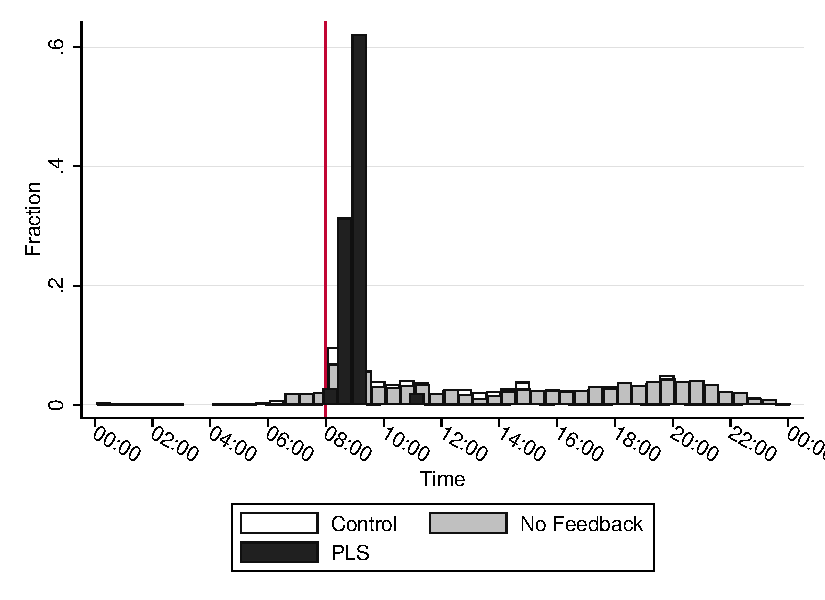
\includegraphics[height=0.8\textheight]{../../figures/hist-deposits.pdf}
		\label{fig:hist-deposits}
		\caption*{\footnotesize \emph{Notes:} This figure plots the empirical distribution of timing of all deposits over the project period. Each bin spans 30 minutes with a height equal to the fraction of all deposits within each treatment group. A vertical line marks 8:00, when participants received the first SMS that summarized how much the participant saved the previous day, how much the participant earned through a matching contribution or winnings, and their total balance. An hour later, participants received a second SMS encouraging them to save that day. Participants in PLS received a new lottery ticket with the second message.}
		\end{figure}

		% People make deposits right when they get the lottery ticket and when results are announced
		% Together this suggests that it's the lottery resolution that matters.

\end{frame}

\begin{frame}{Results}
	
	\centering \large III. What are the effects of PLS on expenditures and savings by other means?

\end{frame}

\begin{frame}{Results -- Other Savings}

	\begin{table}[h]\centering \def\sym#1{\ifmmode^{#1}\else\(^{#1}\)\fi} \caption{Treatment effects -- Savings outside the project} \label{tab:reg-save} \maxsizebox*{\textwidth}{\textheight}{ \begin{threeparttable} \begin{tabular}{l*{5}{c}} \toprule
          &\multicolumn{3}{c}{Effect estimates}&\multicolumn{2}{c}{Sample}\\\cmidrule(lr){2-4}\cmidrule(lr){5-6}
          &\multicolumn{1}{c}{(1)}&\multicolumn{1}{c}{(2)}&\multicolumn{1}{c}{(3)}&\multicolumn{1}{c}{(4)}&\multicolumn{1}{c}{(5)}\\
          &\multicolumn{1}{c}{Lottery}&\multicolumn{1}{c}{Regret}&\multicolumn{1}{c}{\specialcell{Regret-\\Lottery}}&\multicolumn{1}{c}{\specialcell{Control Mean\\(SD)}}&\multicolumn{1}{c}{Obs.}\\
\midrule
Total savings last month (USD PPP)&    18.45&   -17.87&   -36.32&    80.31&      284\\
          &  (25.16)&  (14.64)&  (24.06)& (112.74)&         \\
M-Pesa savings last month (USD PPP)&    -5.42&    -6.71&    -1.29&    20.42&      284\\
          &   (6.34)&   (5.49)&   (5.30)&  (44.67)&         \\
ROSCA savings last month (USD PPP)&     1.48&     7.37&     5.89&    22.24&      283\\
          &   (6.76)&   (6.79)&   (7.33)&  (42.18)&         \\
Currently saves with ROSCA&    -0.02&0.14$^{**}$&0.16$^{**}$&     0.54&      284\\
          &   (0.07)&   (0.07)&   (0.07)&   (0.50)&         \\
\bottomrule \end{tabular} \begin{tablenotes}[flushleft] \footnotesize \item \emph{Notes:} Columns 1--3 report OLS estimates of the treatment effect. Standard errors are in parentheses. Columns 4--5 report the mean and SD of the control group and the number observations, respectively. Observations are at the individual level. * denotes significance at 10 pct., ** at 5 pct., and *** at 1 pct. level. \end{tablenotes} \end{threeparttable} } \end{table}

% File produced by reg-main.do with /Users/Justin/Repos/akiba-lottery-pub/data/clean/akiba_wide.dta on 20:13:21 19 Feb 2018 by user Justin on Stata 13.1 with seed X02be4b816237fe6e6a333726618fd6dd00043d82

	% Since we find no effect on savings amount, we wouldn't expect effects here

\end{frame}

\begin{frame}{Results -- Expenditure}

	\begin{table}[h]\centering \def\sym#1{\ifmmode^{#1}\else\(^{#1}\)\fi} \caption{Treatment effects -- Expenditure} \label{tab:reg-cons} \maxsizebox*{\textwidth}{\textheight}{ \begin{threeparttable} \begin{tabular}{l*{5}{c}} \toprule
          &\multicolumn{3}{c}{Effect estimates}&\multicolumn{2}{c}{Sample}\\\cmidrule(lr){2-4}\cmidrule(lr){5-6}
          &\multicolumn{1}{c}{(1)}&\multicolumn{1}{c}{(2)}&\multicolumn{1}{c}{(3)}&\multicolumn{1}{c}{(4)}&\multicolumn{1}{c}{(5)}\\
          &\multicolumn{1}{c}{Lottery}&\multicolumn{1}{c}{Regret}&\multicolumn{1}{c}{\specialcell{Regret-\\Lottery}}&\multicolumn{1}{c}{\specialcell{Control Mean\\(SD)}}&\multicolumn{1}{c}{Obs.}\\
\midrule
Spent balance on food&     0.04&    -0.08&-0.12$^{*}$&     0.28&      284\\
          &   (0.07)&   (0.06)&   (0.06)&   (0.45)&         \\
Spent balance on school&     0.29&     0.17&    -0.13&     0.24&      284\\
          &   (0.24)&   (0.27)&   (0.32)&   (1.11)&         \\
Spent balance on business&     0.13&0.08$^{*}$&    -0.04&     0.06&      284\\
          &   (0.08)&   (0.04)&   (0.09)&   (0.25)&         \\
Spent balance on durable goods&    -0.00&    -0.03&    -0.03&     0.05&      284\\
          &   (0.03)&   (0.03)&   (0.03)&   (0.23)&         \\
Spent balance on repaying loans&     0.04&    -0.00&    -0.04&     0.11&      284\\
          &   (0.05)&   (0.04)&   (0.05)&   (0.31)&         \\
Saved balance&     0.04&     0.05&     0.01&     0.07&      284\\
          &   (0.04)&   (0.04)&   (0.05)&   (0.26)&         \\
\bottomrule \end{tabular} \begin{tablenotes}[flushleft] \footnotesize \item \emph{Notes:} Columns 1--3 report OLS estimates of the treatment effect. Standard errors are in parentheses. Columns 4--5 report the mean and SD of the control group and the number observations, respectively. Observations are at the individual level. * denotes significance at 10 pct., ** at 5 pct., and *** at 1 pct. level. \end{tablenotes} \end{threeparttable} } \end{table}

% File produced by reg-main.do with /Users/Justin/Repos/akiba-lottery-pub/data/clean/akiba_wide.dta on 11:25:30 16 Feb 2018 by user Justin on Stata 13.1 with seed X27e0a1708256a41cdeaf4038df2ac2a9000400f4

\end{frame}


\begin{frame}{Results -- Gambling}
	
	\centering \large IV. What are the effects of PLS on gambling?

\end{frame}

\begin{frame}{Results}{Gambling}

	\begin{table}[h]\centering \def\sym#1{\ifmmode^{#1}\else\(^{#1}\)\fi} \caption{Multinomial treatment effects -- Gambling behavior} \label{tab:reg-mlogfreq} \maxsizebox*{\textwidth}{\textheight}{ \begin{threeparttable} \begin{tabular}{l*{5}{c}} \toprule
          &\multicolumn{4}{c}{Relative risk ratio}&\multicolumn{1}{c}{Sample}\\\cmidrule(lr){2-5}\cmidrule(lr){6-6}
          &\multicolumn{1}{c}{(1)}&\multicolumn{1}{c}{(2)}&\multicolumn{1}{c}{(3)}&\multicolumn{1}{c}{(4)}&\multicolumn{1}{c}{(5)}\\
          &\multicolumn{1}{c}{Constant}&\multicolumn{1}{c}{No Feedback}&\multicolumn{1}{c}{PLS}&\multicolumn{1}{c}{\specialcell{PLS-\\No Feedback}}&\multicolumn{1}{c}{Obs.}\\
\midrule
Gambled less&     0.22&     0.91&     1.69&     1.86&      284\\
          &   (0.06)&   (0.38)&   (0.66)&   (0.76)&         \\
Gambled more&     0.16&     1.62&     3.03&     1.87&      284\\
          &   (0.05)&   (0.69)&   (1.23)&   (0.69)&         \\
\bottomrule \end{tabular} \begin{tablenotes}[flushleft] \footnotesize \item \emph{Notes:} This table reports estimates from a multinomial logit regression of the categorial response on treatment assigment. Each row corresponds to a response category with the baseline value as . Column 1 reports the constant term corresponding to the mean of the control group. Columns 2--3 reports the treatment effect in relative risk ratios compared to the control group. Column 4 reports the difference between the two PLS treatments. Standard errors are in parentheses. Column 5 reports the number of observations in the analytic sample. Observations are at the individual level. \end{tablenotes} \end{threeparttable} } \end{table}

% File produced by reg-mlogit.do with /Users/justin/Repos/akiba-lottery-pub/data/clean/akiba_wide.dta on 19:20:14 12 Aug 2020 by user justin on Stata 13.1 with seed X71d1d353b37e281e006fa26738e26f4500044a1c

	% The relative risk of gambling more also increases by a factor of 3.03 (1.87) for PLS with feedback compared to without feedback. 

\end{frame}

\begin{frame}{Conclusion}

	\begin{wideitemize}
		\item The savings experiment finds that:
		\begin{enumerate}
			\item PLS can increase account usage but not savings per se.
			\item Behavior is consistent with regret aversion.
			% \item Recently experienced regret reinforces subsequent effect.
			\item Little effect on other savings, consumption.
			\item Some evidence that PLS is complementary to gambling.
		\end{enumerate}
		\item Policy implications
		\begin{itemize}
			\item Welfare consequences are not obvious.
			\item Revenue neutral (in expectation) compared to standard subsidies.
			\item Useful from a policy perspective if it encourages habit formation \parencite{schaner_persistent_2018}.
		\end{itemize}
	\end{wideitemize}

\end{frame}

\begin{frame}[allowframebreaks] \frametitle{References}

	\printbibliography

\end{frame}

\appendix

\begin{frame}{Related Literature}
	
	\begin{enumerate}

		\item \textbf{The effect of PLS on savings}: First field experiment in LMIC to study lottery incentives and the first to test for mechanisms.

		\begin{itemize}
			\item In the lab, lotteries effectively increase the savings rate \parencite{atalay_savings_2014,filiz-ozbay_lottery_2015}.
			\item In the field, works over many domains \parencite{dizon_leveraging_2016,gajic_cost-effectiveness_2011,brune_effect_2015,loibl_testing_2016,gertler_long-term_2017}.
		\end{itemize}

		\item \textbf{Regret aversion in economic choice}: First to study regret aversion in the domain of household finance and provide some evidence on dynamic effects.

		\begin{itemize}
			\item Lottery feedback influences play in Dutch postcode lotteries \parencite{zeelenberg_consequences_2004}.
			\item Loser's regret drives overbidding in first price auctions \parencite{filiz-ozbay_auctions_2007}.
			\item Repeated experiences of regret dissuades risky choices and feedback provides learning opportunities \parencite{imas_regret_2016}.
		\end{itemize}

	\end{enumerate}

\end{frame}

\begin{frame}{The Decision to Save with PLS}

	\begin{itemize}

		\item A one-shot decision problem to save under PLS. Denote $f_i$ the payoff for depositing in state $i$ of the lottery draw and $u(f_i)$ the associated VNM utility. 
	
		\item Saving without feedback satisfies

		\begin{align}
			\sum_{i=1}^4 p_i \cdot [u(f_i) + \gamma R(u(f_i) - u(0))] \geq & u(0) \\
			\sum_{i=1}^4 p_i \cdot [u(f_i) + \gamma R(u(f_i) - u(0))] \geq & u(0) + \textcolor{Triton}{ \sum_{i=1}^4 p_i \cdot \gamma R(u(0) - u(f_i)) }
		\end{align}

		\item Under standard assumptions, saving without feedback condition is stricter than always with feedback so marginal individuals will be induced to save when they expect feedback.

		\item Captures the idea that people who don't save may or may not be exposed to regret and that they take this into account ex ante.

		\item Without regret ($\gamma = 0$), there is no effect of lottery feedback.

	\end{itemize}

\end{frame}

\begin{frame}{Financial Inclusion}

	\begin{figure}[H]
		\centering
		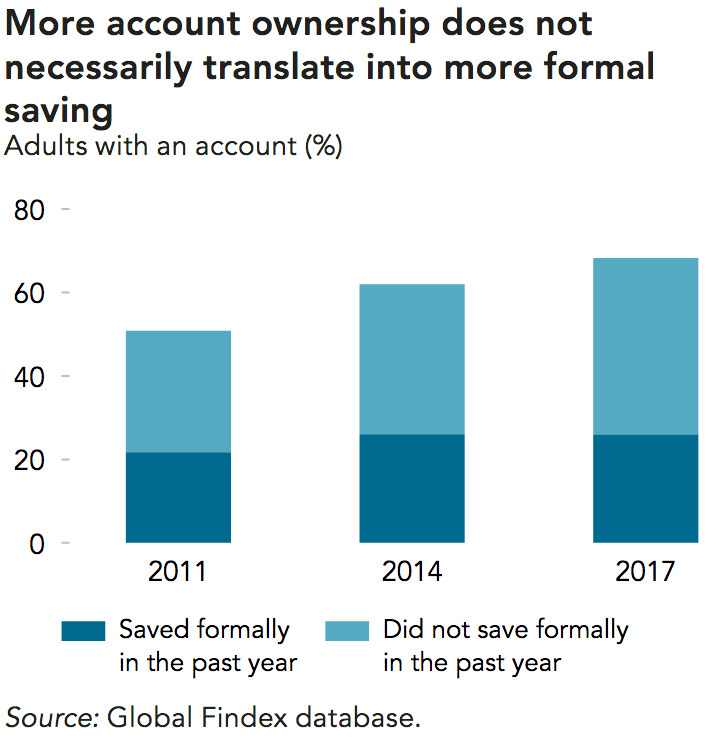
\includegraphics[width=0.45\linewidth]{fig-findex.png}
	\end{figure}

\end{frame}

\begin{frame}{Lottery Draws}

	\begin{table}[htbp]\centering \def\sym#1{\ifmmode^{#1}\else\(^{#1}\)\fi} \caption{Expected and observed lottery results} \label{tab:tab-lottery} \maxsizebox*{\paperwidth}{\paperheight}{ \begin{threeparttable} \begin{tabular}{l*{3}{c}} \toprule
                    &        Freq.&         Pct. observed&      Pct. expected\\
\midrule
No match                   &        7065&       81.49&       62.43\\
One match                   &        1518&       17.51&       22.22\\
Two matches                   &          86&        0.99&       1.23\\
Complete match                   &           1&        0.01&      0.00\\
\bottomrule \end{tabular} \begin{tablenotes}[flushleft] \footnotesize \item \emph{Notes:} The first column tabulates the frequency of observed lottery ticket matches. The second and third columns report the observed and expected probabilities, respectively, of each type of lottery match. A lottery ticket was a random sequence of four numbers between 1 and 9, inclusive. Prizes were awarded according to how well a participant's lottery numbers matched the winning numbers. If the first or second numbers matched, a 10\% match of savings was awarded. If \emph{both} the first and second numbers matched, a 100\% match of savings was awarded. Finally if all numbers matched, a prize of 200 times the daily savings was awarded. \end{tablenotes} \end{threeparttable} } \end{table}


\end{frame}

\begin{frame}{Results -- Regret Aversion}

	We estimate the following equation conditional on assignment to the PLS with feedback group and not having saved one period prior.

	\begin{equation} \begin{split}
		Y_{i,t} = & \pi \text{Win}_{i,t-1} + \omega_{t} + u_{i,t}
	\end{split} \label{eq:regret} \end{equation}

	\begin{align*}
	Y_{i,t}: & i \text{~made a deposit at time~} t \\
	\text{Win}_{i,t-1}: & \text{~won yesterday's lottery} \\
	\omega_t: & \text{~period fixed effect} \\
	u_i: & \text{~idiosyncratic error}
	\end{align*}

\end{frame}

\begin{frame}{Results -- Regret Aversion}
	
	\begin{table}[ht]\centering \def\sym#1{\ifmmode^{#1}\else\(^{#1}\)\fi} \caption{Regression of deposits on lottery results} \label{tab:reg-regretaversion} \maxsizebox*{\textwidth}{\textheight}{ \begin{threeparttable} \begin{tabular}{l*{2}{c}} \toprule
                &\multicolumn{1}{c}{Made a deposit}\\
\midrule
Winning ticket  &     0.02\sym{**} \\
                &   (0.01)         \\
\midrule
Adjusted \(R^{2}\)&    0.081         \\
Control mean    &     0.20         \\
Daily PLS effect&                  \\
Observations    &     4473         \\
\bottomrule \end{tabular} \begin{tablenotes}[flushleft] \footnotesize \item \emph{Notes:} This table reports on a regression of having saved at period \(t\) on winning the lottery at \(t\) conditional on being in the PLS group and not having saved at \(t-1\). The unit of observation is individual-by-period. The regression includes period fixed effects. Standard errors are in parentheses and clustered at the individual level. * denotes significance at 10 pct., ** at 5 pct., and *** at 1 pct. level. \end{tablenotes} \end{threeparttable} } \end{table}

% File produced by akiba-estimate.do with /Users/justin/Repos/akiba-lottery-pub/data/clean/akiba_long.dta on 11:52:17 25 Oct 2020 by user justin on Stata 13.1 with seed Xd950c82044e7d5a124b5a3e57a7d26c000042a30

	% I'm 2% more likely to deposit if I won yesterday than if I lost
	% Foregone winnings from yesterday makes you deposit (play the lottery) today

\end{frame}

\begin{frame}{Results -- Effects Over Time}

	\begin{figure}[H]
		\centering
		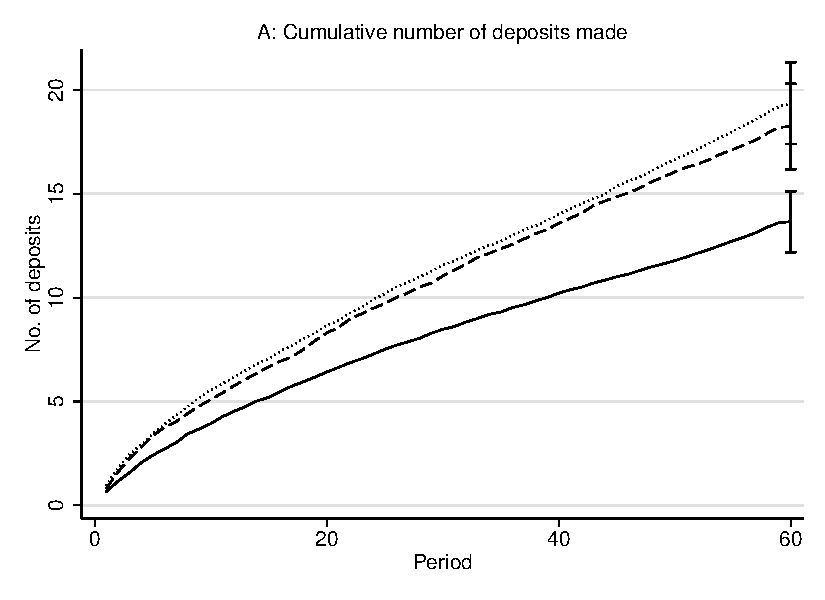
\includegraphics[height=0.8\textheight]{line-mobile_cumdeposits.pdf}
	\end{figure}

\end{frame}

\begin{frame}{Results -- Effects Over Time}

	\begin{figure}[H]
		\centering
		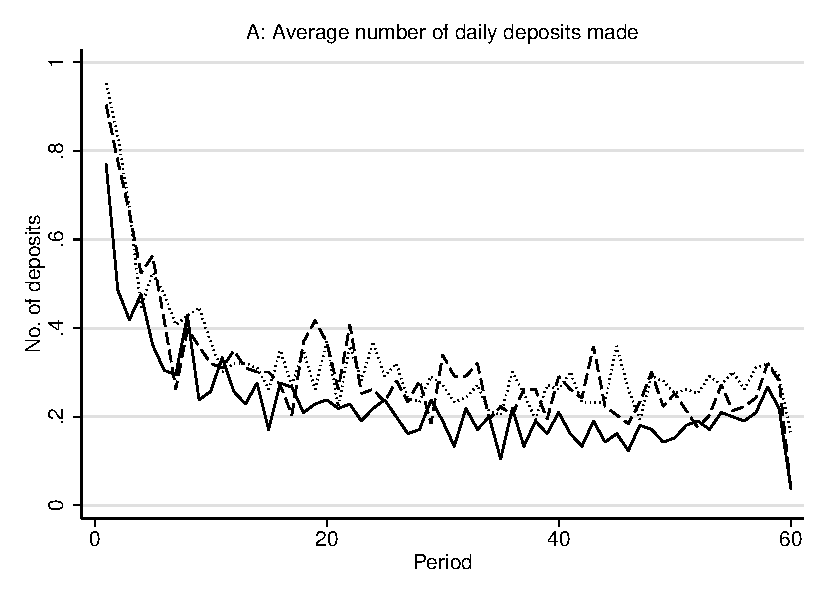
\includegraphics[height=0.8\textheight]{line-mobile_deposits.pdf}
	\end{figure}

\end{frame}

\end{document}

% Notes from 3/13 presentation to graduate students

% What is the most we can say about welfare since the there is a policy focus? There can be an argument made (Gertler et al., Schaner) that habit formation might be a channel. Because it depends on choice architecture, may have to accept that welfare effects are ambiguous. See aer.103.3.387 for a discussion. Given how cheap this is to implement it might be cost-effective.

% x Better explain the insurance product (at least in the presentation)

% x What are other ways subjects could have saved during the time of the study? (esp. mobile credit/savings)? M-Shwari allows people to save using MPESA since 2012. Lockbox account paying an interest of 2-5 percent earned daily for one to six months. Also provides short term credit. Half of all M-Shwari customers do not have any other bank account. In our sample, 31% of subjects use this product. There are no treatment effects on M-Shwari usage. Our product is quite similar to M-Shwari (add as footnote). https://www.cgap.org/sites/default/files/Forum-How-M-Shwari-Works-Apr-2015.pdf

% x The savings variable is a stock so say account balance. Have to check the Z-Tree because maybe this is a flow variable.

% x Explain why we use a lockbox account and explain how we might expect this to affect results/generalizability. Don't assume people are aware of this feature. (Ashraf, Dupas, Aker). This is a common feature of savings products in LIMAC. We chose it because of its ubiquity and demonstrated demand. Why do people value illiquid? Present bias with sophistication, kinship taxes, etc.

% For generalizability: explain where and whether we think this product could work

% Examine the initial dropoff in the plot: is this compositional (extensive margin) or at the intensive margin?

Perhaps it’s useful to mention what airtime / M-Pesa is when presenting to broader audience? I didn’t know what they are before I learned some dev econ. 

The ‘Experiment’ slide (8/28) is a bit hard to read because of the arrangement. Honestly I didn’t understand the difference between PLS and PLS w/o feedback until Ken asked the question and you explained it. Perhaps you can think of a better way to contrast the differences between the three groups?  

Do you have basline information about whether the participants play gambles? If people are just paying to play a 60-day gamble by maintaining balance, perhaps exlcuding those who are more prone to play gamble would change the results? -> Scratch it you just showed us the results. 

For me this paper is more about verifying the regret aversion rather than facilitating savings, but you were motivating the audience with more emphasis given to the savings story. 

Internet connection is really bad, btw… 

Ken: if the expected returns are the same between PLS and PLS w/o feedback, why would people play one rather than the other?
